\section{Appendix} 

\setcounter{table}{0}
\setcounter{figure}{0}
\renewcommand{\thetable}{A\arabic{table}}
\renewcommand{\thefigure}{A\arabic{figure}}

In the following sections we present the equations and methods used for calculating the model set sizes for different model sets under different conditions. To calculate the size of the different model sets, we use the binomial coefficients to calculate the number of possible combinations. The general form of the binomial coefficient is written as
\[\left( \begin{array}{c}
n \\ 
k \end{array}
\right)=\frac{n!}{k!\left(n-k\right)!}\] 
where $n$ is the number of elements which in our case is the number of covariates ($z$) that we want to include, and $k$ is the number of elements taken out. $!$ is the factorial operator, so $n!=n\times \left(n-1\right)\times \left(n-2\right)\times \left(n-3\right)\times \dots \times 3\times 2\times 1$. The binomial coefficient therefore gives us the number of ways that $k$ elements can be chosen from a set of size $n$. One rule that has been repeatedly used is that we can rewrite the sum of binomial coefficients excluding the empty set i.e., not including $i=0$, as 
\[\sum^n_{i=1}{\left( \begin{array}{c}
n \\ 
i \end{array}
\right)}=2^n-1\] 
\\
If we include the empty set this becomes
\[\sum^n_{i=0}{\left( \begin{array}{c}
n \\ 
i \end{array}
\right)}=2^n\] 
\\
When calculating the size of each model set, we consider two different cases; a case without restrictions where we allow interactions without the corresponding main effects, and a case with restrictions where main effects always follow interactions. This means that the second case will be a subset of the first case. \\

% section
\subsection{Model sets without restrictions}
\subsubsection{Set $x + z$}
To calculate the size of the sets, we use the binomial coefficient. The set $x + z$ contains all the combinations that can be made by the covariates $z$ including the model where there is only the variable of interest $x$. Based on the previous terminology the model containing only the variable of interest is therefore the empty set and the binomial coefficient therefore computes how many combinations there are. Let us denote the number of covariates $n$. If we, for example, have three covariates ($n=3$), then the number of combinations where all three covariates are present can be written using the binomial coefficient as
\[\left( \begin{array}{c}
3 \\ 
3 \end{array}
\right)=\frac{3!}{3!\left(3-3\right)!}=1\]
If only two covariates are included in the model from the set of three possible covariates, then the number of combinations becomes 
\[\left( \begin{array}{c}
3 \\ 
2 \end{array}
\right)=\frac{3!}{2!\left(3-2\right)!}=3\] 
And the same if only one covariate is present
\[\left( \begin{array}{c}
3 \\ 
1 \end{array}
\right)=\frac{3!}{1!\left(3-1\right)!}=3\] 
Finally, where no covariates are present, the number of possible combinations is computed as follows
\[\left( \begin{array}{c}
3 \\ 
0 \end{array}
\right)=\frac{3!}{0!\left(3-0\right)!}=1\] 
The total number of models in this set will then be the sum of all these


\[\#\ of\ models\ in\ x + z = \left( \begin{array}{c}
3 \\ 
3 \end{array}
\right)+\left( \begin{array}{c}
3 \\ 
2 \end{array}
\right)+\left( \begin{array}{c}
3 \\ 
1 \end{array}
\right)+\left( \begin{array}{c}
3 \\ 
0 \end{array}
\right)=\sum^3_{i=0}{\left( \begin{array}{c}
3 \\ 
i \end{array}
\right)}\] 
Using the rule for adding binomial coefficients, we can rewrite this into
\[\#\ of\ models\ in\ x + z = \sum^3_{i=0}{\left( \begin{array}{c}
3 \\ 
i \end{array}
\right)}=\left(2^3\right)=8\] 
We can generalize this to the case with $n$ covariates  as follows 
\[\#\ of\ models\ in\ x + z\sum^n_{i=0}{\left( \begin{array}{c}
n \\ 
i \end{array}
\right)}=\left(2^n\right)\] 

\subsubsection{Formally Written} Let $Z$ be the set of covariates 
\[Z=\{\left.z_1,z_2,..,z_n\right.\}\] 
\[\left|Z\right|=n\] 


\noindent The $x + z$ set is then the power set of \emph{Z} 
\[x + z = \{\left.S:S\subseteq Z\right.\}\] 

Each element $S\in x + z$ is a set of the covariates e.g., $S=\left.z_3,z_7\right.$, or any combination of the covariates, including the empty set. This is just the power set of $Z$ and the size of the set can be written as
\[\left|x + z\right|=|\mathcal{P}\left(Z\right)|=2^n\] 
% section
\subsubsection{Set $x \times z$}
The same line of reasoning goes for the $x \times z$ set as for $x + z$ set and we therefore only write it formally. Here, we need to calculate the number of possible interactions between the variable of interest and the covariates. This set will therefore have the same size as the $x + z$ set, as there are as many covariates as there are two-way combinations between the variable of interest and the covariates excluding the empty set.

\[I_h(Z)=\left.\left\{\{x,z_i\}\right.:z_i\in Z\right.\}\] 
\[x \times z=\left.\{T:T\subseteq I_h\left(Z\right),T\neq \textrm{\O}\right.\}\] 
The total number of models in this set is the power set excluding the empty set
\[\left|x \times z\right|\boldsymbol{=}2^n-1\] 

% section
\subsubsection{Set $z \times z$}
The $z \times z$ set contains all combinations of all two-way interactions between the covariates. We first calculate the number of two-way interactions between the covariates and then calculate the number of combinations of these interactions. In the example were $n=3$, the number of two-way interactions is as follows
\[\#\ of\ two-way\ interactions=\left( \begin{array}{c}
3 \\ 
2 \end{array}
\right)=\frac{3!}{2!\left(3-2\right)!}=3\] 
We can then compute the number of combinations of two-way interaction effects using the same method as above 

\noindent 
\[\#\ of\ models\ in\ z \times z=\left( \begin{array}{c}
3 \\ 
3 \end{array}
\right)+\left( \begin{array}{c}
3 \\ 
2 \end{array}
\right)+\left( \begin{array}{c}
3 \\ 
1 \end{array}
\right)=\sum^3_{i=1}{\left( \begin{array}{c}
3 \\ 
i \end{array}
\right)}=7\] 
In general, we can define the number of two-way interactions $h$ that can be generated with $n$ covariates as
\[h=\left( \begin{array}{c}
n \\ 
2 \end{array}
\right)=n(n-1)/2\] 
and the general term for the total number of models in $z \times z$ as
\[\#\ of\ models\ in\ z \times z=\sum^{n(n-1)/2}_{i=1}{\left( \begin{array}{c}
n(n-1)/2 \\ 
i \end{array}
\right)}=(2^{n(n-1)/2}-1)=2^h-1\] 


\subsubsection{Formally written}
Let $Z$ be a set of covariates 
$Z=\{z_1,z_2,..,z_n\}$
\[I_k\left(Z\right)=\{\{\left.\left.z_i,z_j\right.\}:z_i\in Z,z_j\in Z,z_i\neq z_j\right.\}\] 
\[\left|I_k\left(Z\right)\right|=\left( \begin{array}{c}
n \\ 
2 \end{array}
\right)=\frac{n\left(n-1\right)\left(n-2\right)!}{\left(n-2\right)!}\frac{1}{2}=n(n-1)/2\] 
The set of all combinations of two-way interactions between the covariates is then all the subsets of $I_k\left(Z\right)$ excluding the empty set
\[P\left(I_k\left(Z\right)\right)=\{\left.J:J\subseteq I_k\left(Z\right),J\neq \textrm{\O}\right.\}\] 
\[\left|z \times z\right|=\left|P\left(I_k\left(Z\right)\right)\right|=2^{\left|I_k\left(Z\right)\right|}-1=2^{n(n-1)/2}-1\] 
defining 
\[h=\left( \begin{array}{c}
n \\ 
2 \end{array}
\right)=n(n-1)/2\] \\
We can write the number of models in $z \times z$ as
\[\left|z \times z\right|=2^h-1\] \\

% section
\subsubsection{Full model set}
For the following sets: $x + z + x \times z$ , $x + z + z \times z$, and $x + z + x \times z$ + $z \times z$, the equations follow directly from the previous equations as these sets are the products of the previously calculated sets. 

\[\# of\ models\ in\ x + z =\left(2^n\right)\] 
\[\# of\ models\ in\ x \times z=\left(2^n-1\right)\] 
\[\# of\ models\ in\ z \times z=\left(2^h-1\right)\] 
\[\# of\ models\ in\ x + z + x \times z={\left(2^n-1\right)}^2\] 
\[\# of\ models\ in\ x + z+z \times z=\left(2^n-1\right)\left(2^h-1\right)\] 
\[\# of\ models\ in\ x + z + x \times z+z \times z={\left(2^n-1\right)}^2\left(2^h-1\right)\] 
So the total number of models including all sets then becomes
\begin{equation*}
\begin{aligned}
total\ \# \ of\ models=\\
& \underbrace{\left(2^n\right)}_{x + z}+\underbrace{\left(2^n-1\right)}_{x \times z}+\underbrace{\left(2^h-1\right)}_{z \times z}+\\
&\underbrace{{\left(2^n-1\right)}^2}_{x + z + x \times z}+\underbrace{\left(2^n-1\right)\left(2^h-1\right)}_{x \times z+z \times z}+\underbrace{\left(2^n-1\right)\left(2^h-1\right)}_{x + z+z \times z}+\\
&\underbrace{{\left(2^n-1\right)}^2\left(2^h-1\right)}_{x + z + x \times z+z \times z} 
\end{aligned}
\end{equation*}

% For the case where $n=2$, (as in Table \ref{modelsets2.1} under "Models without restrictions" of the main paper), this gives us
%\[h=\left( \begin{array}{c}
%2 \\ 
%2 \end{array}
%\right)=1\] 
%$total \ \#\ of\ models=\left(2^2\right)+\left(2^2-1\right)+\left(2^1-1\right)+{\left(2^2-1\right)}^2+2\left(2^2-1\right)\left(2^1-1\right)+{\left(2^2-1\right)}^2\left(2^1-1\right)=32$ 

% section
\subsection{Model sets with restrictions}
In the case with restrictions, we enforce that every time there is an interaction term, the corresponding main effect terms are included in the model as in the model below:
\[y=x_1+z_1+x_1z_1\] 

In the previous equation, we have an interaction between our variable of interest $x_1$ and a covariate $z_1$. Therefore, the two corresponding main effects also enter the model. This restriction does not change how we calculate the set size of the $x + z$ set as there are no interactions in it. On the other hand,  the restriction implies that the sets $x \times z$ and $z \times z$ are empty sets as the models in these sets never have main effects following interactions. The first set we then need to calculate is then the set $x + z + x \times z$.

% section
\subsubsection{Set $x + z + x \times z$}
For the sake of simplicity, we begin with the case where $n=3$. The models in this set can be seen in Table \ref{tab:appmodel2}. Here the models are split into three different parts. These are split such that $x + z + x \times z$(1), $x + z + x \times z$(2), and $x + z + x \times z$(3) contain all the models where there are one, two, or three covariates, respectively.\\

%\begin{table}[ht!]
%\caption{}
%\caption*{Overview of the models in the $x + z + x \times z$ set when there are three %covariates and one dependent variable}
%\label{tab:appmodel1}
%\centering
%\begin{tabular}{cc}
%\toprule
%Model set & Models \\ 
%\midrule
%\multirow{19}{*}{$x + z + x \times z$} & $y=x_1+z_1+x_1z_1$\\ &  $y=x_1+z_2+x_1z_2$\\ &  $y=x_1+z_3+x_1z_3$\\ & $y=x_1+z_1+z_2+x_1z_1$\\ & $y=x_1+z_1+z_3+x_1z_1$\\ & $y=x_1+z_3+z_1+x_1z_3$\\ & $y=x_1+z_3+z_2+x_1z_3$\\ & $y=x_1+z_2+z_1+x_1z_2$\\ & $y=x_1+z_2+z_3+x_1z_2$\\ & $y=x_1+z_1+z_2+z_3+x_1z_1$\\ & $y=x_1+z_1+z_2+z_3+x_1z_2$\\ & $y=x_1+z_1+z_2+z_3+x_1z_3$\\ & $y=x_1+z_1+z_2+x_1z_1+x_1z_2$\\ & $y=x_1+z_1+z_3+x_1z_1+x_1z_3$\\ & $y=x_1+z_1+z_2+x_1z_3+x_1z_2$\\ & $y=x_1+z_1+z_2+z_3+x_1z_1+x_1z_2$\\ & $y=x_1+z_1+z_2+z_3+x_1z_1+x_1z_3$\\ & $y=x_1+z_1+z_2+z_3+x_1z_3+x_1z_2$\\ & $y=x_1+z_1+z_2+z_3+x_1z_1+x_1z_2+x_1z_3$\\  
%\bottomrule
%\end{tabular}
%\end{table}

\begin{table}[ht!]
\caption{Example of division of the $x + z + x \times z$ set into three subsets when there are three covariates and one dependent variable. $x + z + x \times z$(1) contains all the models with one covariate as main effect, $x + z + x \times z$(2) all the models with two covariates, and $x + z + x \times z$(3) all the models with three covariates}
\centering\label{tab:appmodel2}
\begin{tabular}{lc}  
\toprule
Set & Models \\
\midrule
\multirow{3}{*}{$x + z + x \times z$(1)} & $y=x_1+z_1+x_1z_1$\\ & $y=x_1+z_2+x_1z_2$\\ & $y=x_1+z_3+x_1z_3$\\ & \\ 
\multirow{9}{*}{$x + z + x \times z$(2)} & $y=x_1+z_1$$+z_2+x_1z_1$\\ & $y=x_1+z_1+z_3+x_1z_1$\\ & $y=x_1+z_3+z_1+x_1z_3$\\ & $y=x_1+z_3+z_2+x_1z_3$\\ & $y=x_1+z_2+z_1+x_1z_2$\\ & $y=x_1+z_2+z_3+x_1z_2$\\ & $y=x_1+z_1+z_2+x_1z_1+x_1z_2$\\ & $y=x_1+z_1+z_3+x_1z_1+x_1z_3$\\ & $y=x_1+z_1+z_2+x_1z_3+x_1z_2$\\  & \\  
\multirow{7}{*}{$x + z + x \times z$(3)} & $y=x_1+z_1+z_2+z_3+x_1z_1$\\ & $y=x_1+z_1+z_2+z_3+x_1z_2$\\ & $y=x_1+z_1+z_2+z_3+x_1z_3$\\ & $y=x_1+z_1+z_2+z_3+x_1z_1+x_1z_2$\\ & $y=x_1+z_1+z_2+z_3+x_1z_1+x_1z_3$\\ & $y=x_1+z_1+z_2+z_3+x_1z_3+x_1z_2$\\ & $y=x_1+z_1+z_2+z_3+x_1z_1+x_1z_2+x_1z_3$\\  
\bottomrule
\end{tabular}
\end{table}

To calculate the size of each of these sets separately, we only need to focus on the number of covariates that enter the model, as per assumption the variable of interest $x_1$ is always present. Let us start with the $x + z + x \times z$(1) set. In this set, there can only be one covariate present at the time; there are therefore three combinations, which can be written as $\binom{3}{1}$. In this set, since there is only one covariate, there is only one interaction term containing that same covariate. As no other combinations can be made, this corresponds to $\binom{1}{1}$. Using the same shorthand notation with the binomial coefficient as above, we can write the number of models in the $x + z + x \times z$(1) set as
\[\#\ of\ models\ in\ x + z + x \times z\textit{(1)}\ =\left( \begin{array}{c}
1 \\ 
1 \end{array}
\right)\left( \begin{array}{c}
3 \\ 
1 \end{array}
\right)=\sum^1_{i=1}{\left( \begin{array}{c}
1 \\ 
i \end{array}
\right)}\left( \begin{array}{c}
3 \\ 
1 \end{array}
\right)=\left(2^1-1\right)\left( \begin{array}{c}
3 \\ 
1 \end{array}
\right)=3\] 
Using this notation is useful when we later have to combine the three sets of $x + z + x \times z$ into one to calculate the total number of models in $x + z + x \times z$.

For the $x + z + x \times z$(2) set, we first need to calculate the number of combinations for the main effect that can be made when there are two covariates present at all times and that is $\binom{3}{2}$. Next we need to calculate the number of combinations of interactions that can be present. As we have two covariates present all the time, these are the ones that can be used in the interaction effects. Since the covariates interact with $x_1$, there can either be one or two interaction effects present. Hence, we have $\binom{2}{1}$ and $\binom{2}{2}$ combinations of the interaction effects possible. Combining the number of covariates with the number of possible interactions we get

\begin{equation*}
\begin{aligned}
\#\ of\ models\ in\ x + z +x \times z\textit{(2)}=\\
& \left( \begin{array}{c}
2 \\ 
1 \end{array}
\right)\left( \begin{array}{c}
3 \\ 
2 \end{array}
\right)+\left( \begin{array}{c}
2 \\ 
2 \end{array}
\right)\left( \begin{array}{c}
3 \\ 
2 \end{array}
\right)=\\
&\sum^2_{i=1}{\left( \begin{array}{c}
2 \\ 
i \end{array}
\right)}\left( \begin{array}{c}
3 \\ 
2 \end{array}
\right)=\left(2^2-1\right)\left( \begin{array}{c}
3 \\ 
2 \end{array}
\right)=9

\end{aligned}
\end{equation*}

The same reasoning goes for the $x + z + x \times z$(3) set; the only difference here is that we have one more covariate. So if we write the combinations that are possible with three covariates in the same way as before, we get
\begin{equation*}
\begin{aligned}
\#\ of\ models\ in\ x + z + x \times z\textit{(3)}=\\
&\left( \begin{array}{c}
3 \\ 
1 \end{array}
\right)\left( \begin{array}{c}
3 \\ 
3 \end{array}
\right)+\left( \begin{array}{c}
3 \\ 
2 \end{array}
\right)\left( \begin{array}{c}
3 \\ 
3 \end{array}
\right)+\left( \begin{array}{c}
3 \\ 
3 \end{array}
\right)\left( \begin{array}{c}
3 \\ 
3 \end{array}
\right)= \\
&\sum^3_{i=1}{\left( \begin{array}{c}
2 \\ 
i \end{array}
\right)}\left( \begin{array}{c}
3 \\ 
2 \end{array}
\right)= \\
&\left(2^3-1\right)\left( \begin{array}{c}
3 \\ 
3 \end{array}
\right)=7
\end{aligned}
\end{equation*}
We can then sum all three sets that is, $x + z + x \times z$(1), $x + z + x \times z$(2), and $x + z + x \times z$(3), to get the size of the $x + z + x \times z$ set
\[\#\ of\ models\ in\ x + z + x \times z=\sum^3_{k=1}{(2^k-1)\left( \begin{array}{c}
3 \\ 
k \end{array}
\right)}\]where $k$ is the number of covariates that enter as main effects, meaning it is an indicator for $x + z + x \times z$(1), $x + z + x \times z$(2) and $x + z + x \times z$(3). For the case with $n$ covariates, this becomes
\[\#\ of\ models\ in\ x + z + x \times z=\sum^n_{k=1}{(2^k-1)\left( \begin{array}{c}
n \\ 
k \end{array}
\right)}\] 
\subsubsection{Formally written}
Let $Z$ be a set of covariates 
\[Z=\{\left.z_1,z_2,\dots ,z_n\right.\}\] \[|Z|=n\] 

Let $J$ be a set of indicators of how many covariates enter the model set as main effects
\[J=\{\left.1,2,3,4,\dots ,n\right.\}\] 
Let $L$ be a subset of $Z$ of size $k$
\[L=\{\left.S:S\subset Z,\left|S\right|=k,k\in J\right.\}\] 
The number of interactions that can be made between a covariate and the variable of interest for a given $k$ is then
\[I_h\left(Z\right)=\{\{\left.\left.z_i,x_1\right.\}:z_i\in L\right.\}\] 
\[\left|I_h\left(Z\right)\right|=k\] 

For each $k$, the number of interactions is just the power set of $Z$ excluding the empty set
\[\left|\mathcal{P}\left(I_h\left(Z\right):I_h\left(Z\right)\neq \textrm{\O}\right)\right|=2^k-1\] 

For each $k$, there is $\left( \begin{array}{c}
n \\ 
k \end{array}
\right)$ combinations of interactions that can be present with the number of covariates $k$. To get the full set, we need to sum over these combinations from $k=1$ to $n$ (with $k=0$ it would not be possible to make any interactions so this one is excluded).
\[\left|x + z + x \times z\right|=\sum^n_{k=1}{\left( \begin{array}{c}
n \\ 
k \end{array}
\right)\left(2^k-1\right)}\] 

% section
\subsubsection{Set $x + z + z \times z$}
Here we can use the same line of reasoning as for the $x + z + x \times z$ set. Let us begin by examining the case where $n=3$ and then develop a more general notion. To make it easier to understand how to calculate the set size, we split this set into subsets as we did above for the $x + z + x \times z$ set. This example can be seen in Table \ref{tab:appmodel4}. 

\begin{table}
\centering
\caption{Division of the $x + z + z \times z$ set into two subsets when there are three covariates and one dependent variable. $x + z + z \times z$(2) contains all the models with two covariates as main effects, and $x + z + z \times z$(3) all the models with three covariates. $x + z + z \times z$(1) is an empty set since at least two covariates are necessary to make an interaction.}
\label{tab:appmodel4}
\begin{tabular}{lc} 
\toprule
Set & Models \\ 
\midrule
\multirow{3}{*}{$x + z + z \times z$(2)} & $y=x_1+z_1+z_2+z_1z_2$\\ & $y=x_1+z_1+z_3+z_1z_3$\\ & $y=x_1+z_2+z_3+z_2z_3$\\ &  \\  
\multirow{7}{*}{$x + z + z \times z$(3)} & $y=x_1+z_1+z_2+z_3+z_1z_2$\\ & $y=x_1+z_1+z_3+z_2+z_1z_3$\\ & $y=x_1+z_2+z_3+z_1+z_2z_3$\\ & $y=x_1+z_1+z_2+z_3+z_1z_2+z_1z_3$\\ & $y=x_1+z_1+z_3+z_2+z_1z_3+z_2z_3$\\ & $y=x_1+z_2+z_3+z_1+z_1z_2+z_2z_3$\\ & $y=x_1+z_1+z_2+z_3+z_1z_2+z_2z_3+z_1z_3$\\ 
\bottomrule
\end{tabular}
\end{table}

A model must always include at least two covariates to fulfil the restriction that main effects follow interactions effects. Therefore, we can divide the $x + z + z \times z$ set into two subsets; the first subset has two covariates present as main effects and the second subset has three covariates present as main effects. The first set, $x + z + z \times z$(2), is the number of combinations that can be made from two out of three covariates, meaning $\binom{3}{2}$, multiplied with the combinations of the two covariates that are included, meaning $\binom{2}{2}$.
\[\#\ of\ models\ in\ x + z + z \times z\textit{(2)} =\left( \begin{array}{c}
3 \\ 
2 \end{array}
\right)\left( \begin{array}{c}
2 \\ 
2 \end{array}
\right)=3\] 
For the second subset, $x + z + z \times z$(3), the first term is the number of combinations that can be made with three covariates so this is $\binom{3}{3}$. We then have to calculate the number of interactions that can be made with the three included covariates. To do that, first we need to calculate the number of two-way interactions that can be made with three covariates and this is $\binom{3}{2}=3$. The total number of models in the set is then the sum of the number of combinations
\[\#\ of\ models\ in\ x + z + z \times z\textit{(3)}=\left( \begin{array}{c}
3 \\ 
3 \end{array}
\right)\left(\left( \begin{array}{c}
3 \\ 
1 \end{array}
\right)+\left( \begin{array}{c}
3 \\ 
2 \end{array}
\right)+\left( \begin{array}{c}
3 \\ 
3 \end{array}
\right)\right)=\left( \begin{array}{c}
3 \\ 
3 \end{array}
\right)\sum^3_{i=1}{\left( \begin{array}{c}
3 \\ 
i \end{array}
\right)}\] 
However, it is only in this example that we sum to $n=3$. In general, this will be the number of pairs that can be made in this subset. The number of pairs can be written as $\left( \begin{array}{c}
n \\ 
2 \end{array}
\right)=\frac{n\left(n-1\right)}{2}$. This then becomes
\[\#\ of\ models\ in\ x + z + z \times z\textit{(3)}=\left( \begin{array}{c}
3 \\ 
3 \end{array}
\right)\sum^3_{i=1}{\left( \begin{array}{c}
3 \\ 
i \end{array}
\right)}=\left( \begin{array}{c}
3 \\ 
3 \end{array}
\right)\sum^{\frac{3\left(3-1\right)}{2}}_{i=1}{\left( \begin{array}{c}
\frac{3\left(3-1\right)}{2} \\ 
i \end{array}
\right)}=\left( \begin{array}{c}
3 \\ 
3 \end{array}
\right)\left(2^{\frac{3\left(3-1\right)}{2}}-1\right)\] 
We can write the first subset in the same way
\[\#\ of\ models\ in\ x + z + z \times z(2)=\left( \begin{array}{c}
3 \\ 
2 \end{array}
\right)=\left( \begin{array}{c}
3 \\ 
2 \end{array}
\right)\left(2^{\frac{2\left(2-1\right)}{2}}-1\right)\] 
Now we just add these two subsets up
\[\#\ of\ models\ in\ x + z + z \times z=\left( \begin{array}{c}
3 \\ 
2 \end{array}
\right)\left(2^{\frac{2\left(2-1\right)}{2}}-1\right)+\left( \begin{array}{c}
3 \\ 
3 \end{array}
\right)\left(2^{\frac{3\left(3-1\right)}{2}}-1\right)=\sum^3_{j=2}{\left( \begin{array}{c}
3 \\ 
j \end{array}
\right)\left(2^{\frac{j\left(j-1\right)}{2}}-1\right)}\] 
We can then generalize this case for $n$ covariates
\[\#\ of\ models\ in\ x + z+z \times z=\sum^n_{j=2}{\left( \begin{array}{c}
n \\ 
j \end{array}
\right)\left(2^{\frac{j\left(j-1\right)}{2}}-1\right)}\] 

\subsubsection{Formally written}
Let $Z$ be a set of covariates 
\[Z=\{\left.z_1,z_2,\dots ,z_n\right.\}\] 
\[|Z|=n\] 
Let $k$ be an indicator of how many covariates are included. Since we are using interactions, $k$ must begin at two. Let $T$ be a set of indicators of the number of covariates beginning at two
\[T=\{\left.2,3,4,\dots ,n\right.\}\] 
Let $L$ be a subset of $Z$ of size $k$
\[L=\{\left.S:S\subset Z,\left|S\right|=k,k\in T\right.\}\] 

The number of interactions that can be made for a given $k$ is then
\[I_k\left(Z\right)=\{\left\{\left.z_i,z_j\right\}:z_i\in L,z_j\in L,z_i\neq z_j\right.\}\] 
For a given $k$, the number of two-way interactions that can be made is then
\[\left|I_k\left(Z\right)\right|=\left( \begin{array}{c}
k \\ 
2 \end{array}
\right)=\frac{k!}{2!\left(k-2\right)!}=\frac{k\left(k-1\right)\left(k-2\right)!}{\left(k-2\right)!}\frac{1}{2}=\frac{k\left(k-1\right)}{2}\] 
We then need the combinations of all the two-way interactions. For all $k$, we can take the power set of $I_k\left(H\right)$ excluding the empty set
\[P\left(I_k\left(Z\right)\right)=\{\left.T:T\subset I_k\left(Z\right),T\neq \textrm{\O}\right.\}\] 
\[\left|P\left(I_k\left(Z\right)\right)\right|=2^{\left|I_k\left(Z\right)\right|}-1=2^{\frac{k\left(k-1\right)}{2}}-1\] 
With $n$ covariates, there exist $\left( \begin{array}{c}
n \\ 
k \end{array}
\right)$ subsets of size $k$. To get the $x + z + z \times z$ set, we need to sum over the number of covariates $k$ starting from $k=2$
\[\left|x + z+z \times z\right|=\sum^n_{k=2}{\left( \begin{array}{c}
n \\ 
k \end{array}
\right)}\left(2^{\frac{k\left(k-1\right)}{2}}-1\right)\ \] 

% section
\subsubsection{Set $x + z + x \times z$ + $z \times z$}
This set is the product of the $x + z + x \times z$ and $x + z + z \times z$ sets, but without including the main effect twice. Hence, the set consists of the combinations that can be made between the variable of interest and the covariates and between the covariates alone. We can therefore write 
\[\#\ of\ models\ in\ x + z + x \times z+\ z \times z=\sum^n_{k=2}{\left( \begin{array}{c}
n \\ 
k \end{array}
\right)\left(2^k-1\right)\left(2^{\frac{k\left(k-1\right)}{2}}-1\right)}\] 
\subsubsection{Formally written}
The design of the subsets is the same as earlier and we need to take the product of
$P\left(I_k\left(Z\right)\right)$ and $P\left(I_h\left(Z\right)\right)$, as defined above, and sum over $k$ beginning at two.
For $n$ covariates, there exists $\left( \begin{array}{c}
n \\ 
k \end{array}
\right)$ subsets of size $k$. We then need to sum the subsets as follows
\[|x + z + x \times z+z \times z|=\sum^n_{k=2}{\left( \begin{array}{c}
n \\ 
k \end{array}
\right)\left(2^k-1\right)\left(2^{\frac{k\left(k-1\right)}{2}}-1\right)}\] 

% section
\subsection{Full model set with restrictions}
We now have the full set of models in the $n$ covariate case written as \textbf{HAR TILFØJET SÅ DET STÅR HVAD SET ER HVAD}
\begin{equation} 
\begin{aligned}
\#\ models={} & \underbrace{\left(2^n\right)}_{x + z}+\underbrace{\sum^n_{k=1}{\left(2^k-1\right)\binom{n}{k}}}_{x + z + x \times z} + \\ 
& \underbrace{\sum^n_{k=2}{\binom{n}{j}\left(2^{\frac{k\left(k-1\right)}{2}}-1\right)}}_{x + z + z \times z} + \\
& \underbrace{\sum^n_{k=2}{\binom{n}{k}\left(2^k-1\right)\left(2^{\frac{k\left(k-1\right)}{2}}-1\right)}}_{x + z + x \times z + z \times z}\ \  
\end{aligned}
\end{equation} 

\clearpage
% section
%\subsection{Number of Models}
%In the case without restrictions where we allow interactions without including the corresponding main effects, the total number of models per each set given the number of covariates can be seen in Table \ref{FullModel} under "Without restrictions" in the main paper. For the case with restrictions, the total number of models per each set can be found in either Table \ref{FullModel} in the main part of the manuscript under "With restrictions". 


%\section{Model set for machine learning}
%When researchers are not interested in one specific variable but rather the overall prediction of a given model, such as in machine learning, the same terminology for the sets as used previously can be used to calculate the size of the model sets. 
%As is the case with hypothesis testing, researchers can either demand that main effects are always present when having interactions or they can relax this restriction. \\

%\subsection{When no restrictions are in place}
%In this case, there are three possible sets: $z$, $z \times z$, and $ z + z \times z$. In this case there is no variable that needs to be present all the time as earlier ($x_1$). The calculations of the model set sizes are nevertheless similar to the example with two covariates with no restrictions (see Supplementary Material Case 1 - No Restrictions), and this can be seen in Table \ref{tab:appmodel5} and equation \ref{eq:model1}, \ref{eq:model2} and \ref{eq:model3}.  

%\begin{table}
%\caption{Models for the set $z$, $z \times z$ and $ z + z \times z$ that can be made with two covariates when there is no specific variable of interest. $c$ is a constant, whereas $z_1$ and $z_2$ are covariates}
%\label{tab:appmodel5}
%\centering
%\begin{tabular}{lc} 
%\toprule
%Set & Models \\ 
%\midrule
%\multirow{4}{*}{z} & $y=c$\\ & $y=c + z_1$\\ & $y=c + z_2$\\ & $y=c + z_1 + z_2$\\ &  \\  
%\multirow{1}{*}{$z \times z$} & $y=c + z_1z_2$\\  & \\ 
%\multirow{3}{*}{$x + z + z \times z$}  & $y=c + z_1 + z_1z_2$\\ & $y=c + z_2 + z_1z_2$\\ & $y=c + z_1 + z_2 + z_1z_2$\\ &  \\  
%\bottomrule
%\end{tabular}
%\end{table}

%The calculation for the set size is done as in "Case 1 - No Restrictions"

%\begin{equation}
%\label{eq:model1}
%  \# of\ models\ in\  z\left(2^n\right)
%\end{equation}
%\begin{equation}
%\label{eq:model2}
%  \# of\ models\ in\ z \times z=\left(2^h-1\right)
%\end{equation}
%\begin{equation}
%\label{eq:model3}
%  # of models\ in\ z+z \times z=\left(2^n-1\right)\left(2^h-1\right)
%\end{equation}

%where $h=\left( \begin{array}{c}
%n \\ 
%2 \end{array}
%\right)$. 

%The total number of models given the different number of covariates can be seen in Table \ref{tab:appmodel6}. These calculations apply only when allowing for two-way interactions, but this framework can easily be expanded to include higher order interactions. \\

%% latex table generated in R 4.0.0 by xtable 1.8-4 package
% Wed Dec 30 11:47:49 2020
\begin{table}[!h]
\centering
\caption{} 
\begin{tabular}{rrrrr}
  \hline
Number of covariates & ME & CCI & ME+CCI & Number of models \\ 
  \hline
2 & 4 & 1 & 3 & 8 \\ 
  3 & 8 & 4 & 49 & 61 \\ 
  4 & 16 & 32 & 945 & 993 \\ 
  5 & 32 & 512 & 31713 & 32257 \\ 
  6 & 64 & 16384 & 2064321 & 2080769 \\ 
   \hline
\end{tabular}
\end{table}


%\subsection{When restrictions are in place}
%The calculations here are the same as previously described. However, the only sets that are of interest here are the z and $ z + z \times z$ sets.\\
%The number of models in this case is then \\

%\[\# of models\ in\  z\left(2^n\right)\] 
%\[\# of models\ in\  z+z \times z=\sum^n_{k=2}{\left( %\begin{array}{c}
%n \\ 
%k \end{array}
%\right)}\left(2^{\frac{k\left(k-1\right)}{2}}-1\right)\ \]  

%The total number of models per each model set given the different number of covariates can be seen in Table \ref{tab:appmodel7}.

%% latex table generated in R 4.0.0 by xtable 1.8-4 package
% Wed Dec 30 11:38:43 2020
\begin{table}[!h]
\centering
\caption{} 
\begin{tabular}{rrrr}
  \hline
Number of covariates & ME & ME+CCI & Number of models \\ 
  \hline
2 & 4 & 1 & 5 \\ 
  3 & 8 & 10 & 18 \\ 
  4 & 16 & 97 & 113 \\ 
  5 & 32 & 1418 & 1450 \\ 
  6 & 64 & 40005 & 40069 \\ 
   \hline
\end{tabular}
\end{table}


% section
\subsection{Correlation matrix for simulation}
The following correlation matrix is used for the simulating data with one dependent variable. 

\begin{table}[H]
\centering
\caption{Correlation matrix for the simulated data when having only one dependent variable. r denotes the different correlations set between the covariates and dependent variable in the simulation}
\label{tab:correlation}
\begin{tabular}{c|ccccccc} 
\toprule
 & y & $x_1$ & $z_1$ & $z_2$ & $z_3$ & ... & $z_n$ \\ 
 \midrule
y & 1 &  &  &  &  &  &  \\ 
$x_1$ & 0 & 1 &  &  &  &  &  \\ 
$z_1$ & r & 0 & 1 &  &  &  &  \\  
$z_2$ & r & 0 & 0 & 1 &  &  &  \\  
$z_3$ & r & 0 & 0 & 0 & 1 &  &  \\  
... & r & 0 & 0 & 0 & 0 & 1 &  \\ 
$z_n$ & r & 0 & 0 & 0 & 0 & 0 & 1 \\ 
\bottomrule
\end{tabular}
\end{table}


\clearpage

\subsection{FPP and FPR across model sets}
Table \ref{tab:resultFull} shows the FPP and FPR for the full model sets under different conditions. This is the average effect when using all models at the same time.

% latex table generated in R 4.0.0 by xtable 1.8-4 package
% Wed Oct 28 11:08:01 2020
\begin{longtable}{llrlrrrr}
\caption{} \\ 
  \hline
Main & Type & Sample & Outlier & Correlation & Number of Variables & FPP & FPR \\ 
  \hline
FALSE & Normal & 200 & TRUE & 0.20 & 2.00 & 0.16 & 0.05 \\ 
  FALSE & Normal & 200 & TRUE & 0.20 & 3.00 & 0.27 & 0.05 \\ 
  FALSE & Binomial & 200 & TRUE & 0.20 & 2.00 & 0.75 & 0.16 \\ 
  FALSE & Binomial & 200 & TRUE & 0.20 & 3.00 & 0.91 & 0.15 \\ 
  FALSE & Normal & 300 & TRUE & 0.20 & 2.00 & 0.16 & 0.05 \\ 
  FALSE & Normal & 300 & TRUE & 0.20 & 3.00 & 0.26 & 0.05 \\ 
  FALSE & Binomial & 300 & TRUE & 0.20 & 2.00 & 0.89 & 0.21 \\ 
  FALSE & Binomial & 300 & TRUE & 0.20 & 3.00 & 0.98 & 0.20 \\ 
  FALSE & Normal & 400 & TRUE & 0.20 & 2.00 & 0.16 & 0.05 \\ 
  FALSE & Normal & 400 & TRUE & 0.20 & 3.00 & 0.25 & 0.05 \\ 
  FALSE & Binomial & 400 & TRUE & 0.20 & 2.00 & 0.96 & 0.26 \\ 
  FALSE & Binomial & 400 & TRUE & 0.20 & 3.00 & 1.00 & 0.24 \\ 
  FALSE & Normal & 200 & TRUE & 0.30 & 2.00 & 0.20 & 0.06 \\ 
  FALSE & Normal & 200 & TRUE & 0.30 & 3.00 & 0.36 & 0.06 \\ 
  FALSE & Binomial & 200 & TRUE & 0.30 & 2.00 & 0.99 & 0.28 \\ 
  FALSE & Binomial & 200 & TRUE & 0.30 & 3.00 & 1.00 & 0.28 \\ 
  FALSE & Normal & 300 & TRUE & 0.30 & 2.00 & 0.20 & 0.06 \\ 
  FALSE & Normal & 300 & TRUE & 0.30 & 3.00 & 0.35 & 0.06 \\ 
  FALSE & Binomial & 300 & TRUE & 0.30 & 2.00 & 1.00 & 0.34 \\ 
  FALSE & Binomial & 300 & TRUE & 0.30 & 3.00 & 1.00 & 0.35 \\ 
  FALSE & Normal & 400 & TRUE & 0.30 & 2.00 & 0.21 & 0.06 \\ 
  FALSE & Normal & 400 & TRUE & 0.30 & 3.00 & 0.33 & 0.06 \\ 
  FALSE & Binomial & 400 & TRUE & 0.30 & 2.00 & 1.00 & 0.37 \\ 
  FALSE & Binomial & 400 & TRUE & 0.30 & 3.00 & 1.00 & 0.39 \\ 
  FALSE & Normal & 200 & FALSE & 0.20 & 2.00 & 0.16 & 0.05 \\ 
  FALSE & Normal & 200 & FALSE & 0.20 & 3.00 & 0.27 & 0.05 \\ 
  FALSE & Binomial & 200 & FALSE & 0.20 & 2.00 & 0.75 & 0.16 \\ 
  FALSE & Binomial & 200 & FALSE & 0.20 & 3.00 & 0.92 & 0.15 \\ 
  FALSE & Normal & 300 & FALSE & 0.20 & 2.00 & 0.16 & 0.05 \\ 
  FALSE & Normal & 300 & FALSE & 0.20 & 3.00 & 0.25 & 0.05 \\ 
  FALSE & Binomial & 300 & FALSE & 0.20 & 2.00 & 0.89 & 0.21 \\ 
  FALSE & Binomial & 300 & FALSE & 0.20 & 3.00 & 0.98 & 0.20 \\ 
  FALSE & Normal & 400 & FALSE & 0.20 & 2.00 & 0.16 & 0.05 \\ 
  FALSE & Normal & 400 & FALSE & 0.20 & 3.00 & 0.25 & 0.05 \\ 
  FALSE & Binomial & 400 & FALSE & 0.20 & 2.00 & 0.96 & 0.25 \\ 
  FALSE & Binomial & 400 & FALSE & 0.20 & 3.00 & 1.00 & 0.24 \\ 
  FALSE & Normal & 200 & FALSE & 0.30 & 2.00 & 0.21 & 0.05 \\ 
  FALSE & Normal & 200 & FALSE & 0.30 & 3.00 & 0.35 & 0.06 \\ 
  FALSE & Binomial & 200 & FALSE & 0.30 & 2.00 & 0.99 & 0.28 \\ 
  FALSE & Binomial & 200 & FALSE & 0.30 & 3.00 & 1.00 & 0.28 \\ 
  FALSE & Normal & 300 & FALSE & 0.30 & 2.00 & 0.20 & 0.06 \\ 
  FALSE & Normal & 300 & FALSE & 0.30 & 3.00 & 0.34 & 0.06 \\ 
  FALSE & Binomial & 300 & FALSE & 0.30 & 2.00 & 1.00 & 0.34 \\ 
  FALSE & Binomial & 300 & FALSE & 0.30 & 3.00 & 1.00 & 0.34 \\ 
  FALSE & Normal & 400 & FALSE & 0.30 & 2.00 & 0.20 & 0.05 \\ 
  FALSE & Normal & 400 & FALSE & 0.30 & 3.00 & 0.34 & 0.06 \\ 
  FALSE & Binomial & 400 & FALSE & 0.30 & 2.00 & 1.00 & 0.37 \\ 
  FALSE & Binomial & 400 & FALSE & 0.30 & 3.00 & 1.00 & 0.39 \\ 
  TRUE & Normal & 200 & TRUE & 0.20 & 2.00 & 0.13 & 0.05 \\ 
  TRUE & Normal & 200 & TRUE & 0.20 & 3.00 & 0.20 & 0.05 \\ 
  TRUE & Binomial & 200 & TRUE & 0.20 & 2.00 & 0.14 & 0.05 \\ 
  TRUE & Binomial & 200 & TRUE & 0.20 & 3.00 & 0.22 & 0.04 \\ 
  TRUE & Normal & 300 & TRUE & 0.20 & 2.00 & 0.12 & 0.05 \\ 
  TRUE & Normal & 300 & TRUE & 0.20 & 3.00 & 0.18 & 0.05 \\ 
  TRUE & Binomial & 300 & TRUE & 0.20 & 2.00 & 0.14 & 0.05 \\ 
  TRUE & Binomial & 300 & TRUE & 0.20 & 3.00 & 0.22 & 0.05 \\ 
  TRUE & Normal & 400 & TRUE & 0.20 & 2.00 & 0.12 & 0.05 \\ 
  TRUE & Normal & 400 & TRUE & 0.20 & 3.00 & 0.19 & 0.05 \\ 
  TRUE & Binomial & 400 & TRUE & 0.20 & 2.00 & 0.14 & 0.05 \\ 
  TRUE & Binomial & 400 & TRUE & 0.20 & 3.00 & 0.21 & 0.04 \\ 
  TRUE & Normal & 200 & TRUE & 0.30 & 2.00 & 0.14 & 0.05 \\ 
  TRUE & Normal & 200 & TRUE & 0.30 & 3.00 & 0.23 & 0.05 \\ 
  TRUE & Binomial & 200 & TRUE & 0.30 & 2.00 & 0.16 & 0.05 \\ 
  TRUE & Binomial & 200 & TRUE & 0.30 & 3.00 & 0.26 & 0.05 \\ 
  TRUE & Normal & 300 & TRUE & 0.30 & 2.00 & 0.14 & 0.05 \\ 
  TRUE & Normal & 300 & TRUE & 0.30 & 3.00 & 0.23 & 0.05 \\ 
  TRUE & Binomial & 300 & TRUE & 0.30 & 2.00 & 0.15 & 0.04 \\ 
  TRUE & Binomial & 300 & TRUE & 0.30 & 3.00 & 0.25 & 0.05 \\ 
  TRUE & Normal & 400 & TRUE & 0.30 & 2.00 & 0.14 & 0.05 \\ 
  TRUE & Normal & 400 & TRUE & 0.30 & 3.00 & 0.22 & 0.05 \\ 
  TRUE & Binomial & 400 & TRUE & 0.30 & 2.00 & 0.16 & 0.05 \\ 
  TRUE & Binomial & 400 & TRUE & 0.30 & 3.00 & 0.26 & 0.05 \\ 
  TRUE & Normal & 200 & FALSE & 0.20 & 2.00 & 0.12 & 0.05 \\ 
  TRUE & Normal & 200 & FALSE & 0.20 & 3.00 & 0.19 & 0.05 \\ 
  TRUE & Binomial & 200 & FALSE & 0.20 & 2.00 & 0.14 & 0.04 \\ 
  TRUE & Binomial & 200 & FALSE & 0.20 & 3.00 & 0.22 & 0.04 \\ 
  TRUE & Normal & 300 & FALSE & 0.20 & 2.00 & 0.13 & 0.05 \\ 
  TRUE & Normal & 300 & FALSE & 0.20 & 3.00 & 0.19 & 0.05 \\ 
  TRUE & Binomial & 300 & FALSE & 0.20 & 2.00 & 0.14 & 0.05 \\ 
  TRUE & Binomial & 300 & FALSE & 0.20 & 3.00 & 0.22 & 0.04 \\ 
  TRUE & Normal & 400 & FALSE & 0.20 & 2.00 & 0.12 & 0.05 \\ 
  TRUE & Normal & 400 & FALSE & 0.20 & 3.00 & 0.19 & 0.05 \\ 
  TRUE & Binomial & 400 & FALSE & 0.20 & 2.00 & 0.14 & 0.05 \\ 
  TRUE & Binomial & 400 & FALSE & 0.20 & 3.00 & 0.21 & 0.04 \\ 
  TRUE & Normal & 200 & FALSE & 0.30 & 2.00 & 0.13 & 0.05 \\ 
  TRUE & Normal & 200 & FALSE & 0.30 & 3.00 & 0.23 & 0.05 \\ 
  TRUE & Binomial & 200 & FALSE & 0.30 & 2.00 & 0.16 & 0.05 \\ 
  TRUE & Binomial & 200 & FALSE & 0.30 & 3.00 & 0.27 & 0.05 \\ 
  TRUE & Normal & 300 & FALSE & 0.30 & 2.00 & 0.14 & 0.05 \\ 
  TRUE & Normal & 300 & FALSE & 0.30 & 3.00 & 0.23 & 0.05 \\ 
  TRUE & Binomial & 300 & FALSE & 0.30 & 2.00 & 0.16 & 0.05 \\ 
  TRUE & Binomial & 300 & FALSE & 0.30 & 3.00 & 0.26 & 0.05 \\ 
  TRUE & Normal & 400 & FALSE & 0.30 & 2.00 & 0.14 & 0.05 \\ 
  TRUE & Normal & 400 & FALSE & 0.30 & 3.00 & 0.23 & 0.05 \\ 
  TRUE & Binomial & 400 & FALSE & 0.30 & 2.00 & 0.16 & 0.05 \\ 
  TRUE & Binomial & 400 & FALSE & 0.30 & 3.00 & 0.25 & 0.04 \\ 
   \hline
\hline
\end{longtable}


\clearpage

% section
\subsection{Supporting figures}
In this section are two additional figures illustrating the consequences using several dependent variables and what happens if the correlation between the dependent variable and the covariates increases. Figure \ref{fig:appfigure2app} shows the effect of using two dependent variables and the average of the two (a total of three dependent variables). Everything else is similar to the baseline model in meaning that the sample size is 200, there are two covariates, no outlier deletion and the correlation between the dependent variable and the covariates is $\textit{r}=0.2$.\\
Figure \ref{fig:appfigure1app} shows the effect of increasing the correlation between the dependent variable and the covariates. Here the increase goes from $\textit{r}=0.2$ til $\textit{r}=0.3$ and $\textit{r}=0.4$. Everything else is similar to the baseline model. \\

\begin{figure}[ht!]
%\figuretitle{Effect of using several dependent variables}
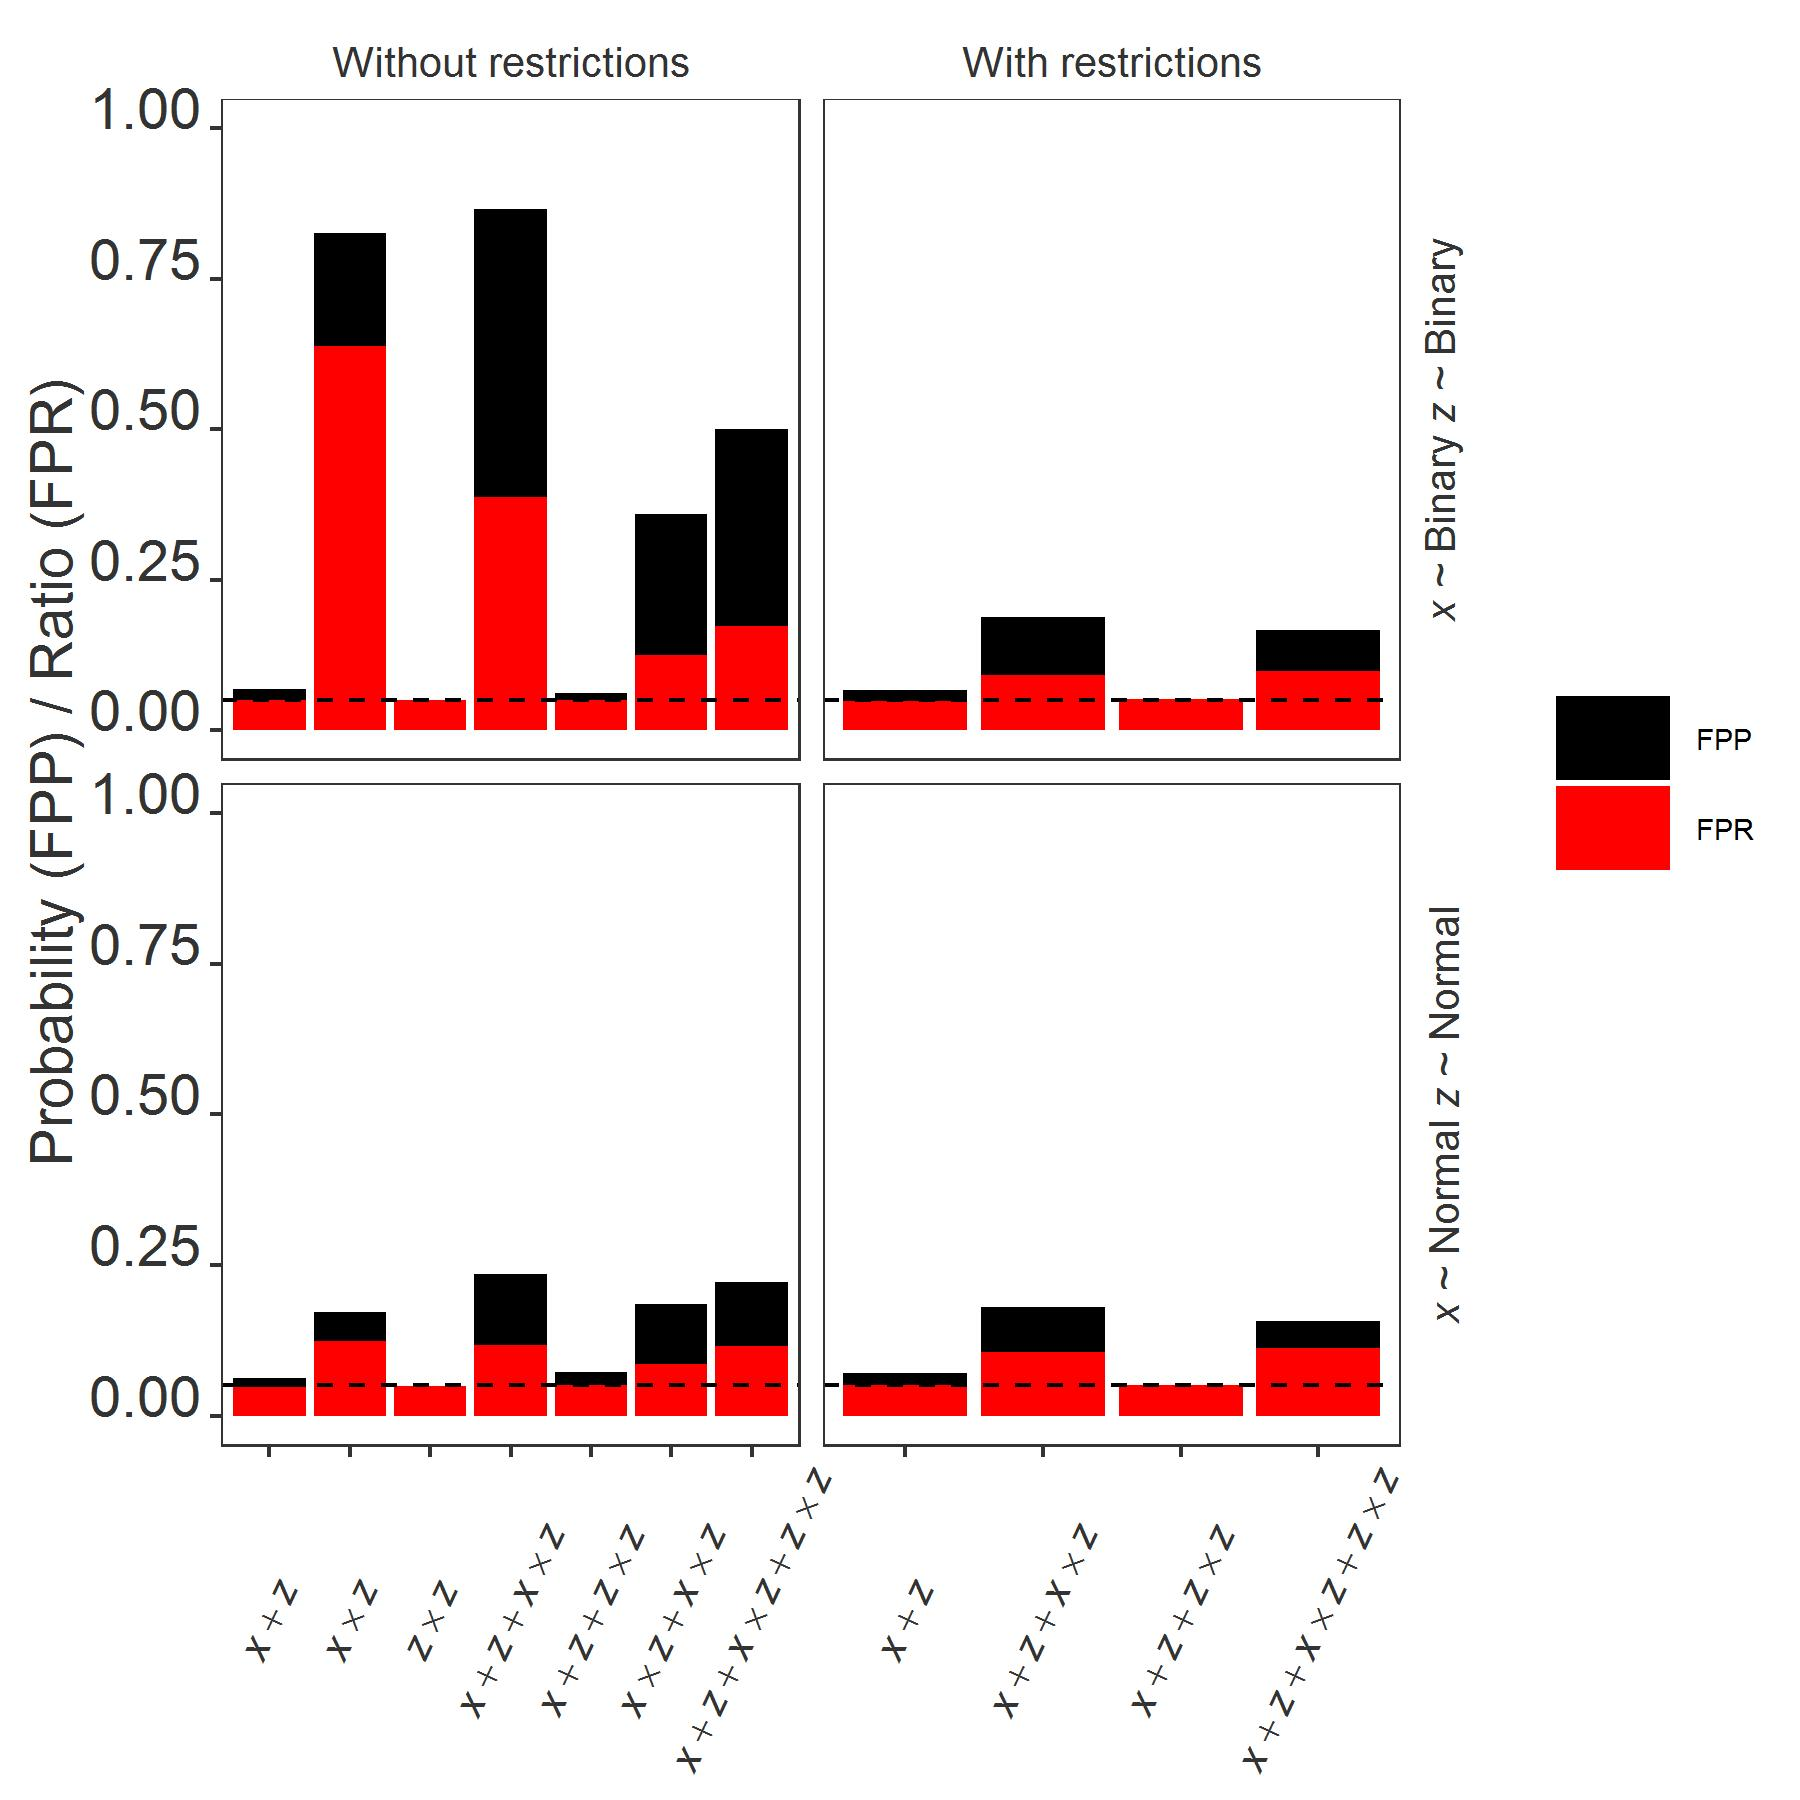
\includegraphics[width=0.7\textwidth]{R/Analysis/Result/Figures/Figure2App.jpeg}
\centering
\caption{false-positive probability and false-positive ratio when using two dependent variables and the average of the two (three dependent variables in total). The correlation between the dependent variables is set to  $\textit{r}=0.5$ with the correlation between the dependent variables and covariates still at  $\textit{r}=0.2$. Black denotes the the false-positive probability and red denotes the false-positive ratio. Dashed blacked line indicates 0.05. The description of the figure is otherwise the same as for Figure \ref{fig:mainfigure1}.}
\label{fig:appfigure2app}
\end{figure}

\begin{figure}[ht!]
%\figuretitle{Effect of increasing the correlation between the dependent variable and the covariates}
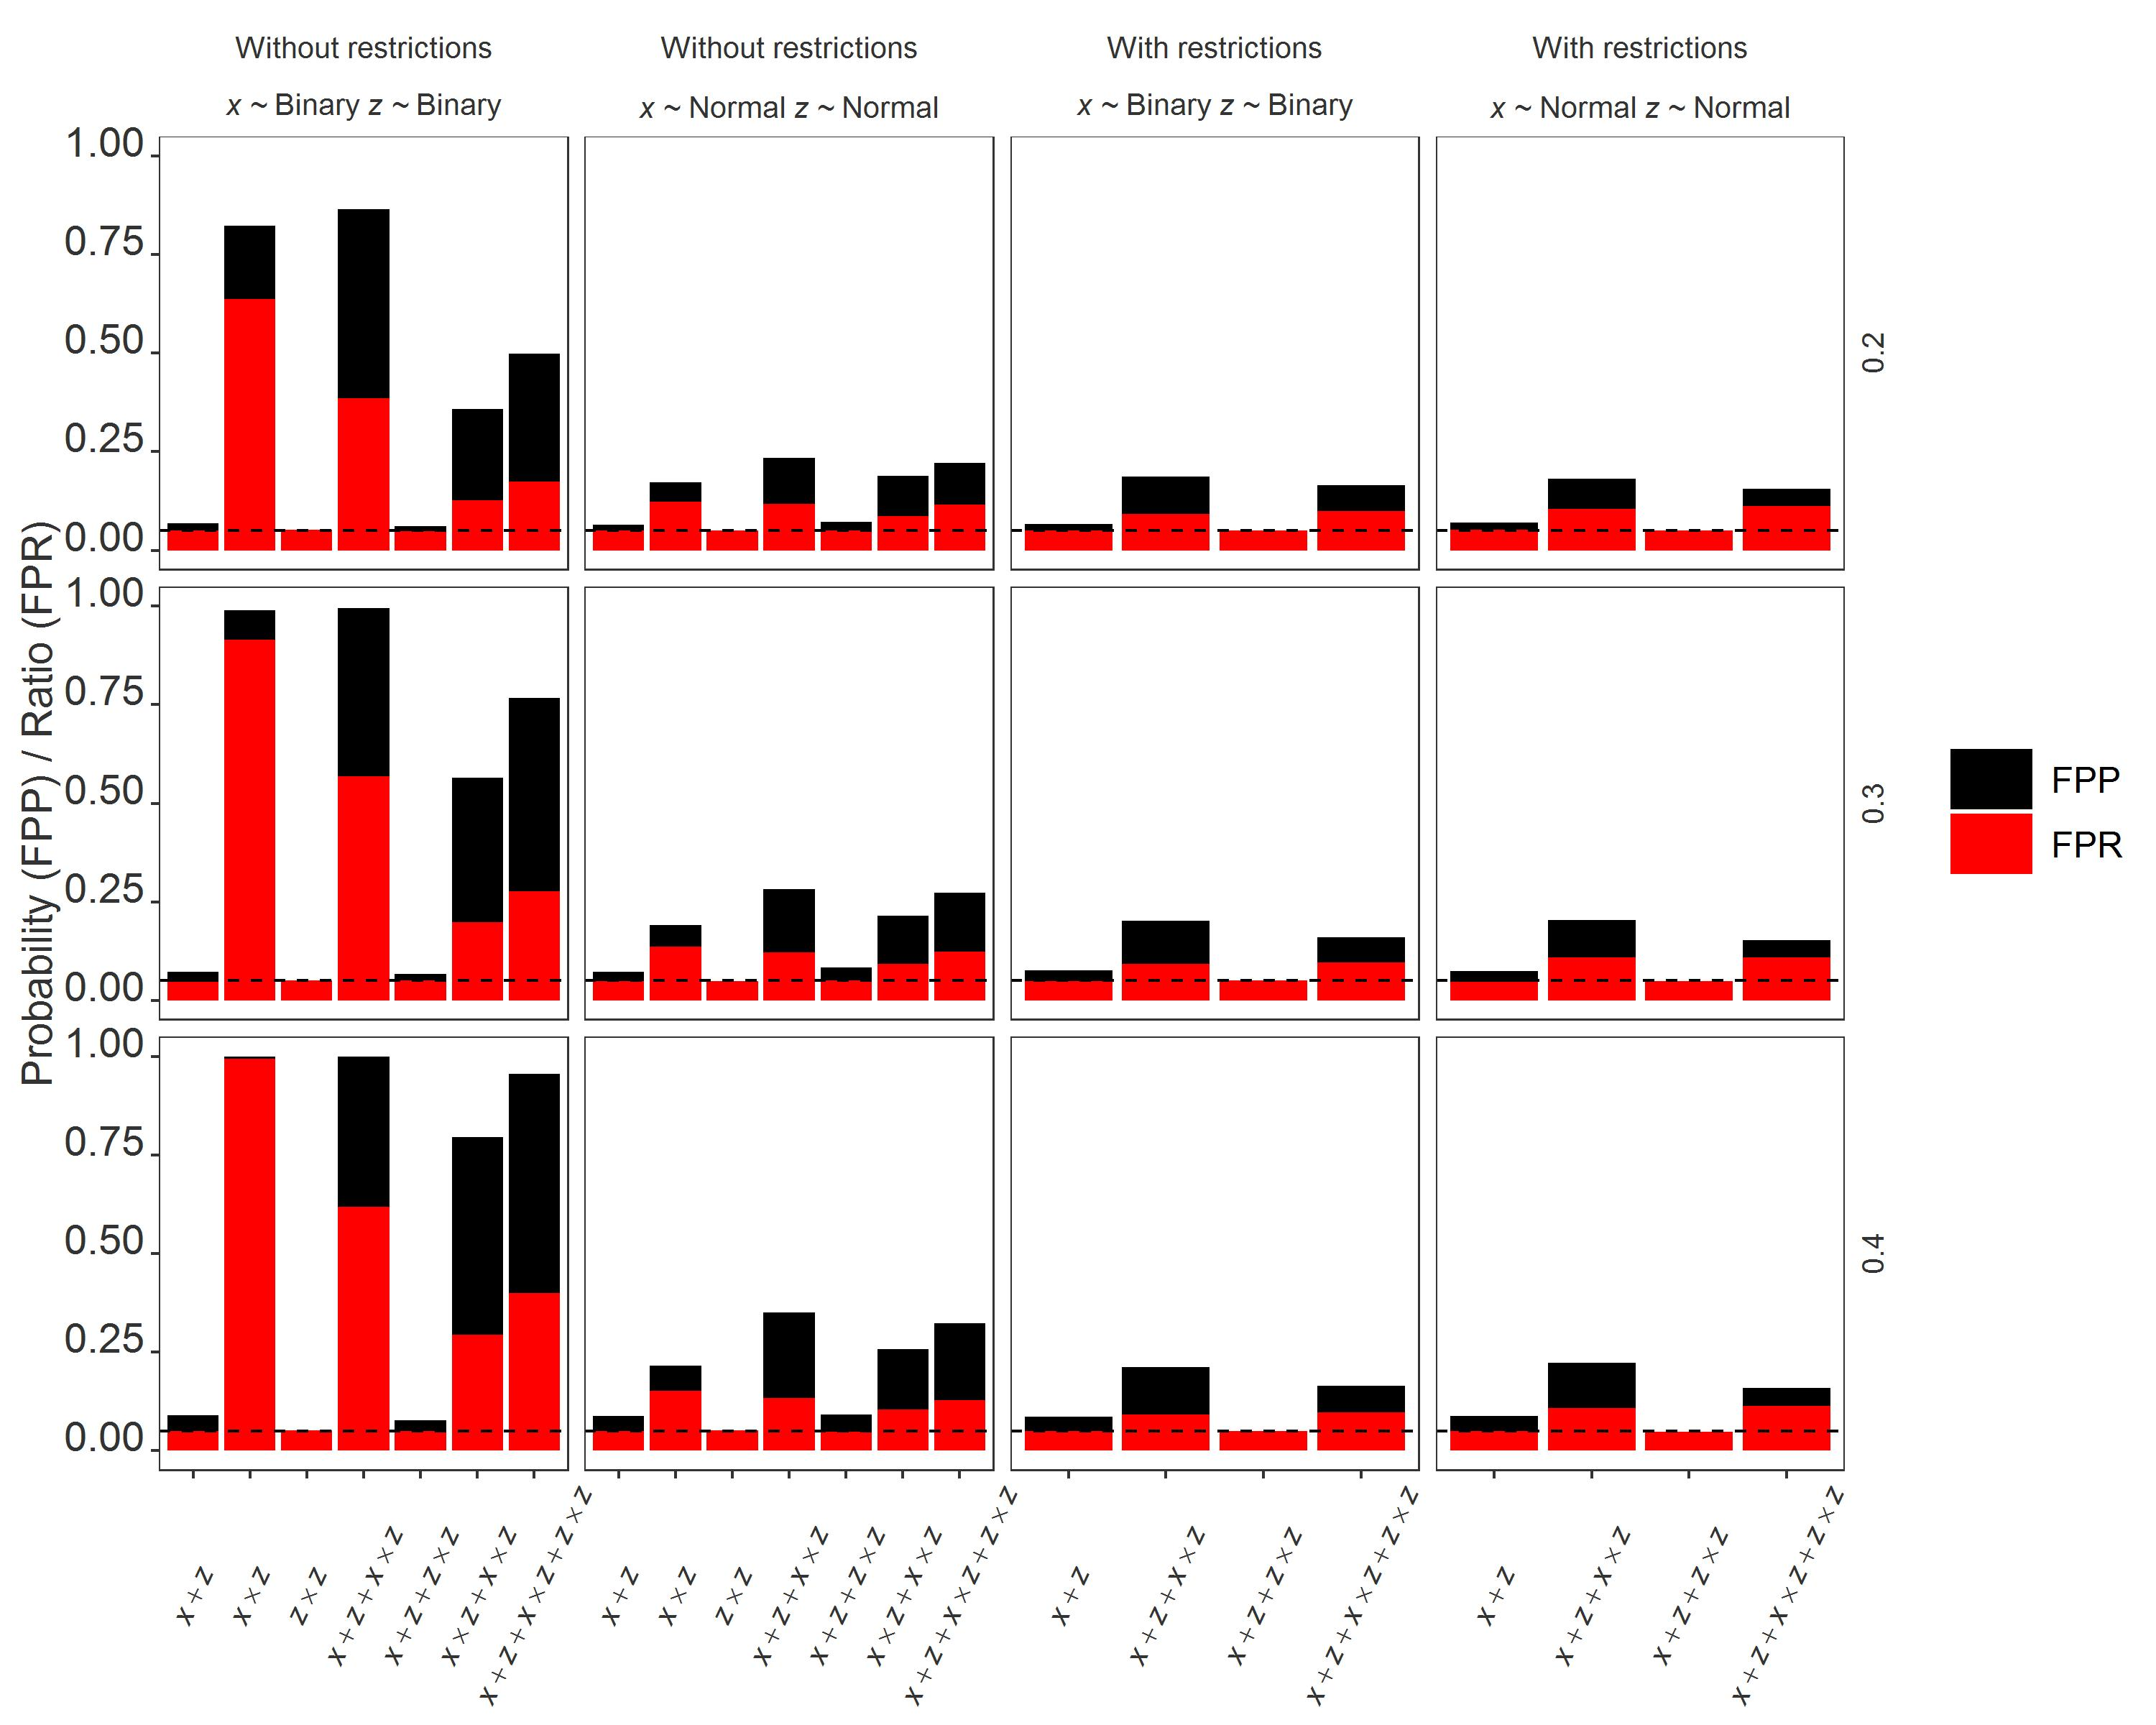
\includegraphics[width=1\textwidth]{R/Analysis/Result/Figures/Figure1App.jpeg}
\centering
\caption{false-positive probability and false-positive for different levels of correlation between the dependent variable and the covariates ranging from  $\textit{r}=0.2$ to  $\textit{r}=0.4$. Black denotes the false-positive probability and red denotes the false-positive ratio. Dashed blacked line indicates 0.05. The description of the figure is otherwise the same as for Figure \ref{fig:mainfigure1}.}
\label{fig:appfigure1app}
\end{figure}



\clearpage
